\documentclass[aspectratio=169]{beamer}

% Theme and colors
\usetheme{Madrid}
\usecolortheme{whale}
\setbeamertemplate{navigation symbols}{}
\setbeamertemplate{footline}[frame number]

% Packages
\usepackage{tikz}
\usetikzlibrary{shapes,arrows,positioning,calc,decorations.pathreplacing}
\usepackage{booktabs}
\usepackage{graphicx}
\usepackage{xcolor}
\usepackage{tcolorbox}
\usepackage{array}

% Custom colors
\definecolor{ipblue}{RGB}{0,51,102}
\definecolor{innovgreen}{RGB}{0,100,50}
\definecolor{warningred}{RGB}{180,0,0}
\definecolor{techgray}{RGB}{64,64,64}
\definecolor{goldaccent}{RGB}{180,140,20}
\definecolor{publicdomain}{RGB}{70,130,180}

% Custom blocks
\newtcolorbox{argumentbox}[1][]{
  colback=ipblue!5,
  colframe=ipblue,
  fonttitle=\bfseries,
  title={#1},
  boxrule=1pt,
  arc=2pt
}

\newtcolorbox{quotebox}[1][]{
  colback=gray!10,
  colframe=gray!50,
  fonttitle=\itshape,
  title={#1},
  boxrule=0.5pt,
  arc=2pt,
  left=10pt,
  right=10pt
}

\newtcolorbox{casestudybox}[1][]{
  colback=goldaccent!10,
  colframe=goldaccent,
  fonttitle=\bfseries,
  title={#1},
  boxrule=1pt,
  arc=2pt
}

\newtcolorbox{objectionbox}[1][]{
  colback=warningred!5,
  colframe=warningred,
  fonttitle=\bfseries,
  title={#1},
  boxrule=1pt,
  arc=2pt
}

% Title information
\title[Intellectual Property]{Intellectual Property in the Digital Age}
\subtitle{Creation, Control, and the Battle for Ideas}
\author{Brendan Shea, PhD}
\institute{Rochester Community and Technical College\\Computing and AI Ethics}
\date{}

\begin{document}

% ===== SLIDE 1: Title =====
\begin{frame}
\titlepage
\end{frame}

% ===== SLIDE 2: The Central Question =====
\begin{frame}{The Central Question}
\begin{itemize}
    \item Why should anyone ``\textbf{own}'' an idea?
    \item How do we balance \textbf{creators' rights} with \textbf{public access} to knowledge?
    \item Has intellectual property law kept up with digital technology---or been \textbf{captured} by powerful interests?
\end{itemize}

\vspace{0.4cm}
\begin{quotebox}[Thomas Jefferson, Letter to Isaac McPherson (1813)]
``He who receives an idea from me, receives instruction himself without lessening mine; as he who lights his taper at mine, receives light without darkening me.''
\end{quotebox}

\begin{alertblock}{?}
Have you ever pirated something? Felt guilty about it? Why or why not?
\end{alertblock}
\end{frame}

% ===== SLIDE 3: What is Intellectual Property? =====
\begin{frame}{What is Intellectual Property?}
\textbf{Definition}: Legal rights that protect creations of the mind

\vspace{0.2cm}
\begin{itemize}
    \item \textbf{Intangible}: Unlike physical property, ideas can be copied without ``taking'' them
    \item \textbf{Non-rivalrous}: Your use doesn't prevent my use (unlike a sandwich)
    \item \textbf{Artificial scarcity}: IP law creates scarcity where none naturally exists
    \item \textbf{Time-limited} (usually): Eventually enters the ``public domain''
\end{itemize}

\vspace{0.3cm}
\begin{center}
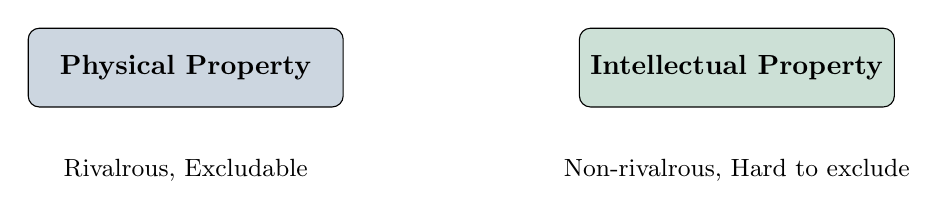
\begin{tikzpicture}
    \node[rectangle, draw, fill=ipblue!20, rounded corners, minimum width=4cm, minimum height=1cm] (physical) at (0,0) {\textbf{Physical Property}};
    \node[rectangle, draw, fill=innovgreen!20, rounded corners, minimum width=4cm, minimum height=1cm] (ip) at (7,0) {\textbf{Intellectual Property}};
    
    \node[below of=physical, yshift=-0.3cm, font=\small] {Rivalrous, Excludable};
    \node[below of=ip, yshift=-0.3cm, font=\small] {Non-rivalrous, Hard to exclude};
\end{tikzpicture}
\end{center}

\vspace{0.2cm}
\textbf{The fundamental tension}: Creators want compensation; society wants access to knowledge.
\end{frame}

% ===== SLIDE 4: The Four Types of IP =====
\begin{frame}{The Four Types of Intellectual Property}
\begin{table}[h]
\centering
\small
\begin{tabular}{>{\bfseries}l p{4cm} l p{3cm}}
\toprule
Type & Protects & Duration & Example \\
\midrule
Copyright & Creative expression (books, music, code) & Life + 70 years (US) & Harry Potter novels \\
Patents & Useful inventions and processes & 20 years & Pharmaceutical drugs \\
Trademarks & Brand identifiers (names, logos) & Indefinite (if renewed) & Nike swoosh \\
Trade Secrets & Confidential business info & Indefinite (if kept secret) & Coca-Cola formula \\
\bottomrule
\end{tabular}
\end{table}

\vspace{0.3cm}
\textbf{Key point}: Each type has \textbf{different justifications}, durations, and rules.

\begin{alertblock}{?}
Which type of IP is most important for the tech industry? Why?
\end{alertblock}
\end{frame}

% ===== SLIDE 5: Copyright in Depth =====
\begin{frame}{Copyright in Depth}
\textbf{What it protects}: Original works of authorship fixed in tangible form

\vspace{0.2cm}
\begin{columns}[T]
\begin{column}{0.48\textwidth}
\textbf{Rights granted}:
\begin{itemize}
    \item Right to \textbf{reproduce}, distribute, display
    \item Right to create \textbf{derivative works}
    \item Right to control who can do the above
\end{itemize}
\end{column}

\begin{column}{0.48\textwidth}
\textbf{What it does NOT protect}:
\begin{itemize}
    \item \textbf{Ideas} themselves (only expression)
    \item \textbf{Facts} and \textbf{functional elements}
    \item Works in the \textbf{public domain}
\end{itemize}
\end{column}
\end{columns}

\vspace{0.3cm}
\textbf{Key limitation}: \textbf{Fair use} doctrine (criticism, education, parody, transformative use)

\begin{alertblock}{?}
If you write a song that sounds exactly like another song but you never heard the original, is that infringement?
\end{alertblock}
\end{frame}

% ===== SLIDE 6: Patents in Depth =====
\begin{frame}{Patents in Depth}
\textbf{What it protects}: Novel, useful, non-obvious inventions

\vspace{0.2cm}
\textbf{Requirements for patent}:
\begin{itemize}
    \item \textbf{Novelty}: Must be new
    \item \textbf{Utility}: Must be useful
    \item \textbf{Non-obviousness}: Can't be obvious to someone skilled in the field
\end{itemize}

\vspace{0.3cm}
\begin{casestudybox}[The Patent Bargain]
\begin{itemize}
    \item Inventor \textbf{discloses} how the invention works (public learns)
    \item In exchange: \textbf{20-year monopoly} on making, selling, and using
\end{itemize}
\end{casestudybox}

\vspace{0.2cm}
\textbf{Types}: Utility patents, design patents, plant patents

\textbf{Key tension}: Encourages innovation vs. blocks follow-on innovation
\end{frame}

% ===== SLIDE 7: Trademarks and Trade Secrets =====
\begin{frame}{Trademarks and Trade Secrets}
\begin{columns}[T]
\begin{column}{0.48\textwidth}
\begin{block}{\textbf{Trademarks}}
\begin{itemize}
    \item Protect \textbf{source identifiers}
    \item Must be \textbf{distinctive} (not generic)
    \item Can last \textbf{forever} if actively used
    \item ``\textbf{Genericide}'': When trademarks become generic (aspirin, escalator, zipper)
\end{itemize}
\end{block}
\end{column}

\begin{column}{0.48\textwidth}
\begin{block}{\textbf{Trade Secrets}}
\begin{itemize}
    \item Protected by \textbf{keeping them secret}
    \item \textbf{No time limit}---but once revealed, protection lost
    \item Examples: Algorithms, customer lists, recipes
    \item Legal protection against \textbf{misappropriation}
\end{itemize}
\end{block}
\end{column}
\end{columns}

\vspace{0.4cm}
\begin{alertblock}{?}
Is it ethical to reverse-engineer a competitor's trade secret?
\end{alertblock}
\end{frame}

% ===== SLIDE 8: A Brief History of IP =====
\begin{frame}{A Brief History of Intellectual Property}
\begin{table}[h]
\centering
\small
\begin{tabular}{l p{9cm}}
\toprule
\textbf{Year} & \textbf{Development} \\
\midrule
1710 & Statute of Anne (first copyright law)---14 years, renewable once \\
1790 & US Copyright Act---14 years \\
1886 & Berne Convention---international copyright harmonization \\
1976 & US Copyright Act---life + 50 years \\
1994 & TRIPS Agreement---links IP to global trade \\
1998 & DMCA + Sonny Bono Act---life + 70 years \\
2020s & AI and streaming reshape everything \\
\bottomrule
\end{tabular}
\end{table}

\vspace{0.2cm}
\textbf{Key observation}: IP terms have \textbf{consistently expanded}, always justified by ``encouraging creativity''---but is that what's actually happening?
\end{frame}

% ===== SLIDE 9: Justification 1: Locke's Labor Theory =====
\begin{frame}{Justification 1: Locke's Labor Theory}
\begin{argumentbox}[The Labor Argument]
\begin{enumerate}
    \item People have a \textbf{natural right} to the fruits of their labor.
    \item Intellectual creations are the product of \textbf{mental labor}.
    \item Therefore, creators have a natural right to \textbf{control their creations}.
\end{enumerate}
\end{argumentbox}

\vspace{0.3cm}
\textbf{The Lockean proviso}: ...as long as ``enough and as good'' is left for others

\vspace{0.3cm}
\textbf{Problems with this view}:
\begin{itemize}
    \item Ideas \textbf{build on prior ideas}---how much is really ``yours''?
    \item Does mixing labor with something give you the \textbf{whole thing}?
    \item Digital copying requires \textbf{no labor} from the copier
\end{itemize}
\end{frame}

% ===== SLIDE 10: Justification 2: Utilitarian Theory =====
\begin{frame}{Justification 2: Utilitarian / Incentive Theory}
\begin{argumentbox}[The Incentive Argument]
\begin{enumerate}
    \item Society benefits from creative works and inventions.
    \item Creating such works requires time, effort, and resources.
    \item Without protection, creators can't recoup their investment (others will copy).
    \item IP rights provide \textbf{incentives} for creation.
    \item[\textbf{C.}] \textbf{Therefore, IP is justified because it maximizes social welfare.}
\end{enumerate}
\end{argumentbox}

\vspace{0.2cm}
\textbf{The dominant view}: This is how courts and legislatures usually justify IP.

\vspace{0.2cm}
\textbf{Critical questions}:
\begin{itemize}
    \item What's the \textbf{optimal length} of protection? (Current terms may exceed what's needed)
    \item Does IP actually \textbf{incentivize}, or mostly enrich incumbents?
    \item What about creation that happens \textbf{without} IP incentives (open source, fan fiction)?
\end{itemize}
\end{frame}

% ===== SLIDE 11: Justification 3: Personality Theory =====
\begin{frame}{Justification 3: Personality / Expression Theory}
\textbf{Associated with}: Hegel, continental European tradition \hfill \textbf{Core idea}: Works are \textbf{extensions of personality}

\vspace{0.1cm}
\begin{argumentbox}[The Personality Argument]
\begin{enumerate}
    \item Persons have \textbf{dignity} and deserve respect for their self-expression.
    \item Creative works \textbf{embody} the creator's personality and vision.
    \item[\textbf{C.}] \textbf{Therefore, creators have moral rights beyond economic rights.}
\end{enumerate}
\end{argumentbox}

\vspace{0.1cm}
\textbf{Moral rights} (droit moral): Right of \textbf{attribution} (credit), right of \textbf{integrity} (no distortion). Stronger in Europe than US.

\begin{alertblock}{?}
Does an AI have ``personality'' that could be expressed in creative works?
\end{alertblock}
\end{frame}

% ===== SLIDE 12: The Social Contract of IP =====
\begin{frame}{The Social Contract of IP}
\textbf{The bargain}: Society grants \textbf{temporary monopoly}; creator gets \textbf{compensation}; public eventually gets access.

\vspace{0.2cm}
\begin{center}
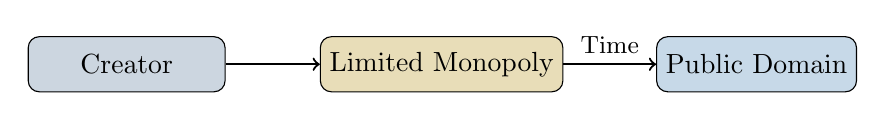
\begin{tikzpicture}[node distance=2cm]
    \node[rectangle, draw, fill=ipblue!20, rounded corners, minimum width=2.5cm, minimum height=0.7cm] (creator) {Creator};
    \node[rectangle, draw, fill=goldaccent!30, rounded corners, minimum width=3cm, minimum height=0.7cm, right of=creator, xshift=2cm] (monopoly) {Limited Monopoly};
    \node[rectangle, draw, fill=publicdomain!30, rounded corners, minimum width=2.5cm, minimum height=0.7cm, right of=monopoly, xshift=2cm] (public) {Public Domain};
    \draw[->, thick] (creator) -- (monopoly);
    \draw[->, thick] (monopoly) -- node[above] {\small Time} (public);
\end{tikzpicture}
\end{center}

\vspace{0.1cm}
\textbf{Is this bargain still working?} Terms keep \textbf{extending}; enforcement \textbf{expanding}; IP concentrating in \textbf{fewer hands}.

\vspace{0.1cm}
\begin{quotebox}[James Boyle, \textit{The Public Domain} (2008)]
``We are in the middle of a second enclosure movement... `the enclosure of the intangible commons of the mind.'\,''
\end{quotebox}
\end{frame}

% ===== PART II HEADER =====
\begin{frame}
\begin{center}
{\Huge \textbf{Part II}}\\[0.5cm]
{\Large The Digital Transformation}\\[0.3cm]
{\large How Technology Broke (and Remade) Intellectual Property}
\end{center}
\end{frame}

% ===== SLIDE 14: How Digital Changed Everything =====
\begin{frame}{How Digital Technology Changed Everything}
\begin{columns}[T]
\begin{column}{0.48\textwidth}
\begin{block}{\textbf{Pre-Digital Reality}}
\begin{itemize}
    \item Copying was \textbf{expensive} and imperfect
    \item Distribution required \textbf{physical infrastructure}
    \item Enforcement was relatively straightforward
\end{itemize}
\end{block}
\end{column}

\begin{column}{0.48\textwidth}
\begin{block}{\textbf{Digital Reality}}
\begin{itemize}
    \item \textbf{Perfect copies} at zero marginal cost
    \item \textbf{Global distribution} instantaneous
    \item Anyone can be a publisher---or a pirate
\end{itemize}
\end{block}
\end{column}
\end{columns}

\vspace{0.4cm}
\textbf{The economic shift}:
\begin{itemize}
    \item Scarcity moves from \textbf{copies} to \textbf{attention}
    \item Value shifts from \textbf{content} to \textbf{platforms}
    \item Old business models collapse
\end{itemize}

\vspace{0.2cm}
\textbf{Key insight}: IP law was designed for a world of \textbf{physical scarcity} that no longer exists.
\end{frame}

% ===== SLIDE 15: The Internet's Challenge =====
\begin{frame}{The Internet's Challenge to Copyright}
\textbf{What the internet did}:
\begin{itemize}
    \item Made everyone a potential \textbf{publisher}
    \item Made copying \textbf{trivially easy}
    \item Made distribution \textbf{global and instant}
    \item Made enforcement nearly impossible at individual level
\end{itemize}

\vspace{0.3cm}
\textbf{Industry responses}:
\begin{itemize}
    \item \textbf{Litigation} (sue individuals, platforms)
    \item \textbf{Legislation} (DMCA, SOPA/PIPA attempts)
    \item \textbf{Technology} (DRM, copy protection)
    \item \textbf{New business models} (streaming, subscriptions)
\end{itemize}

\vspace{0.2cm}
\textbf{The cultural shift}: A generation grew up treating digital content as essentially free.
\end{frame}

% ===== SLIDE 16: Napster Case Study =====
\begin{frame}{Case Study: Napster and the P2P Revolution}
\begin{casestudybox}[Napster (1999--2001)]
\textbf{The facts}: Napster enabled millions to share MP3 files peer-to-peer.

\textbf{The lawsuit}: \textit{A\&M Records v. Napster}---recording industry sued for contributory infringement.

\textbf{The outcome}: Napster shut down in 2001, but technology moved on (Kazaa, BitTorrent, etc.)
\end{casestudybox}

\vspace{0.2cm}
\textbf{The aftermath}: Music industry revenue \textbf{collapsed} (then recovered via streaming); demonstrated that \textbf{law couldn't stop technology}; led to iTunes, Spotify, and the streaming model.

\begin{alertblock}{?}
Did Napster ``kill'' the music industry---or force it to innovate?
\end{alertblock}
\end{frame}

% ===== SLIDE 17: The DMCA =====
\begin{frame}{The DMCA and Digital Locks}
\textbf{The Digital Millennium Copyright Act (1998)}:

\vspace{0.2cm}
\textbf{Key provisions}:
\begin{itemize}
    \item \textbf{Anti-circumvention}: Illegal to break digital locks (DRM), even for legal purposes
    \item \textbf{Safe harbors}: Platforms not liable if they respond to takedown notices
    \item \textbf{Notice and takedown}: Copyright holders can demand removal
\end{itemize}

\vspace{0.3cm}
\textbf{The problem with anti-circumvention}:
\begin{itemize}
    \item Can't rip your own DVDs for backup
    \item Can't unlock your own phone (until exemptions granted)
    \item Security researchers criminalized
    \item \textbf{Right to repair} blocked
\end{itemize}

\vspace{0.2cm}
\textbf{Key insight}: DMCA shifted power from \textbf{owners} to \textbf{manufacturers}.
\end{frame}

% ===== SLIDE 18: Streaming Model =====
\begin{frame}{Streaming and the New Distribution Model}
\textbf{The shift}: From \textbf{ownership} to \textbf{access}

\vspace{0.1cm}
\textbf{How streaming changed IP}: Users don't ``own'' content---they \textbf{rent access}. Platforms can \textbf{remove content at will}. Artists earn fractions of a cent per play. Catalog value concentrated in \textbf{platforms}, not creators.

\vspace{0.1cm}
\begin{table}[h]
\centering
\small
\begin{tabular}{l l}
\toprule
\textbf{Metric} & \textbf{Value} \\
\midrule
Spotify pay per stream & \$0.003--\$0.005 (varies by country) \\
Streams needed for \$1 & 200--330 streams \\
Minimum threshold (2024) & 1,000 streams/year to earn anything \\
\bottomrule
\end{tabular}
\end{table}

\textbf{Who won?} Platforms and major labels, not necessarily artists or consumers.

\begin{alertblock}{?}
Is ``access to everything'' better than ``owning some things''?
\end{alertblock}
\end{frame}

% ===== PART III HEADER =====
\begin{frame}
\begin{center}
{\Huge \textbf{Part III}}\\[0.5cm]
{\Large Critiques and Abuses of IP}\\[0.3cm]
{\large When Protection Becomes Predation}
\end{center}
\end{frame}

% ===== SLIDE 20: Peter Drahos =====
\begin{frame}{Peter Drahos: Information Feudalism}
\textbf{Key work}: \textit{Information Feudalism: Who Owns the Knowledge Economy?} (2002, with John Braithwaite)

\vspace{0.2cm}
\textbf{Core argument}:
\begin{itemize}
    \item IP has been \textbf{globalized} through trade agreements (TRIPS, etc.)
    \item Driven by small number of \textbf{powerful corporations}, not public interest
    \item Creates new feudal relationships: \textbf{IP lords and IP serfs}
    \item Developing countries forced to adopt strong IP regimes
\end{itemize}

\vspace{0.3cm}
\textbf{The mechanism}:
\begin{itemize}
    \item Link IP to \textbf{trade agreements}
    \item Threaten \textbf{trade sanctions} for non-compliance
    \item \textbf{Ratchet up} protection globally
\end{itemize}

\vspace{0.2cm}
\textbf{Key insight}: IP expansion is about \textbf{market control}, not innovation.
\end{frame}

% ===== SLIDE 21: Cory Doctorow =====
\begin{frame}{Cory Doctorow: Chokepoint Capitalism}
\textbf{Key work}: \textit{Chokepoint Capitalism} (2022, with Rebecca Giblin)

\vspace{0.2cm}
\textbf{Core argument}:
\begin{itemize}
    \item Big Tech and Big Content have created ``\textbf{chokepoints}''---bottlenecks they control
    \item IP law helps \textbf{maintain} these chokepoints
    \item Creators are squeezed between powerful buyers and sellers
    \item The problem isn't piracy---it's \textbf{monopsony} (buyer power)
\end{itemize}

\vspace{0.3cm}
\textbf{Examples of chokepoints}:
\begin{itemize}
    \item \textbf{Amazon} controls book/ebook market
    \item \textbf{Spotify} controls streaming
    \item \textbf{Google/Apple} control app distribution
    \item \textbf{Audible} controls audiobooks (with DRM lock-in)
\end{itemize}

\vspace{0.2cm}
\textbf{The solution}: Not stronger IP, but \textbf{competition policy} and \textbf{interoperability mandates}.
\end{frame}

% ===== SLIDE 22: Tim Wu =====
\begin{frame}{Tim Wu: IP and the Attention Economy}
\textbf{Key works}: \textit{The Master Switch}, \textit{The Attention Merchants}

\vspace{0.2cm}
\textbf{Core insights}:
\begin{itemize}
    \item Communication technologies follow a cycle: \textbf{open $\rightarrow$ closed $\rightarrow$ regulated $\rightarrow$ disrupted}
    \item IP is a tool for \textbf{maintaining closure}
    \item \textbf{Attention} is the real scarce resource; IP controls access to attention
\end{itemize}

\vspace{0.3cm}
\textbf{The pattern}:
\begin{enumerate}
    \item New technology promises \textbf{openness}
    \item Incumbents use IP to establish \textbf{control}
    \item \textbf{Consolidation} follows
    \item Until next \textbf{disruption}
\end{enumerate}

\vspace{0.2cm}
\textbf{Application to Big Tech}: Platforms use IP (and IP-adjacent tools like ToS, APIs) to maintain dominance.
\end{frame}

% ===== SLIDE 23: Disney Case Study =====
\begin{frame}{Case Study: Disney and Copyright Extension}
\begin{casestudybox}[Mickey Mouse and Copyright]
\textbf{The pattern}: 1928: Mickey appears in ``Steamboat Willie'' $\rightarrow$ 1976: Copyright Act extends terms $\rightarrow$ 1998: Sonny Bono Act extends again $\rightarrow$ \textbf{Jan 1, 2024}: Steamboat Willie finally enters public domain
\end{casestudybox}

\vspace{0.2cm}
\textbf{The lobbying}: Disney among largest lobbyists for copyright extension; Sonny Bono Act sometimes called ``Mickey Mouse Protection Act.''

\vspace{0.1cm}
\textbf{The critique}: \textbf{Retroactive extension} can't incentivize creation already done---pure rent-seeking.

\vspace{0.1cm}
\textbf{The catch}: Disney still holds \textbf{trademarks} on Mickey and copyrights on \textbf{later versions}.

\begin{alertblock}{?}
Should corporations be able to own characters indefinitely through trademark?
\end{alertblock}
\end{frame}

% ===== SLIDE 24: Pharma Case Study =====
\begin{frame}{Case Study: Pharmaceutical Patents and Access to Medicine}
\begin{casestudybox}[The Pharma IP Problem]
Drug development is expensive (\$1--2B per approved drug). Patents grant \textbf{20-year monopoly pricing}. Result: Life-saving drugs priced beyond reach of many.
\end{casestudybox}

\vspace{0.2cm}
\textbf{Examples}: HIV/AIDS drugs initially \$10,000+/year, generics \textasciitilde\$100/year. Insulin prices in US often 10x higher than other countries. EpiPen price increases 600\%+ over time.

\vspace{0.2cm}
\textbf{The tension}:
\begin{itemize}
    \item Without patents, less incentive for R\&D (utilitarian argument)
    \item With patents, people die from lack of access (harm)
\end{itemize}

\textbf{The global dimension}: TRIPS agreement forces developing countries to respect pharma patents.
\end{frame}

% ===== SLIDE 25: Patent Trolls =====
\begin{frame}{Case Study: Patent Trolls and Strategic Litigation}
\begin{casestudybox}[Patent Trolls (Non-Practicing Entities)]
\textbf{What is a patent troll?}
\begin{itemize}
    \item Companies that own patents but \textbf{don't make products}
    \item Business model: Sue or threaten to sue actual producers
    \item Target: Often \textbf{small companies} who can't afford litigation
\end{itemize}
\end{casestudybox}

\vspace{0.2cm}
\textbf{The economics}:
\begin{itemize}
    \item Average patent lawsuit costs \$2--5 million to defend
    \item Settling for \$100K--500K is ``rational'' even if you'd win
    \item Trolls acquire vague patents cheaply, extract settlements
\end{itemize}

\vspace{0.2cm}
\textbf{Example}: Personal Audio LLC sued podcasters over ``episodic content distribution'' patents.

\vspace{0.2cm}
\textbf{The harm}: Innovation tax; discourages small innovators; resources wasted on litigation.
\end{frame}

% ===== SLIDE 26: Enshittification =====
\begin{frame}{The ``Enshittification'' Connection}
\textbf{Doctorow's concept}: Platforms decay in a predictable pattern

\vspace{0.2cm}
\textbf{The cycle}: (1) Platform is \textbf{good to users} $\rightarrow$ (2) \textbf{good to business customers} $\rightarrow$ (3) \textbf{extracts value} from both

\vspace{0.2cm}
\textbf{How IP enables enshittification}:
\begin{itemize}
    \item \textbf{DRM and lock-in}: Can't leave with your purchases
    \item \textbf{ToS as law}: Platforms can change rules unilaterally
    \item \textbf{API control / Copyright claims}: Cut off competitors, silence criticism
\end{itemize}

\textbf{Key insight}: IP isn't just about protecting creation---it's about \textbf{controlling markets}.

\begin{alertblock}{?}
Have you experienced enshittification? Which platforms?
\end{alertblock}
\end{frame}

% ===== PART IV HEADER =====
\begin{frame}
\begin{center}
{\Huge \textbf{Part IV}}\\[0.5cm]
{\Large Big Tech and Platform IP}\\[0.3cm]
{\large How Tech Giants Weaponize Intellectual Property}
\end{center}
\end{frame}

% ===== SLIDE 28: How Big Tech Uses IP =====
\begin{frame}{How Big Tech Uses IP}
\textbf{The arsenal}:

\begin{table}[h]
\centering
\small
\begin{tabular}{>{\bfseries}l p{7.5cm}}
\toprule
Tool & How It's Used \\
\midrule
Patents & Build defensive portfolios; sue competitors; cross-license with other giants \\
Copyright & Control user content; DMCA takedowns; protect code \\
Trade secrets & Algorithms, training data, business methods \\
Trademarks & Brand protection; keyword advertising disputes \\
Terms of Service & Create IP-like control without formal IP \\
\bottomrule
\end{tabular}
\end{table}

\vspace{0.2cm}
\textbf{The strategy}:
\begin{itemize}
    \item Accumulate IP for \textbf{defense and offense}
    \item Use IP to \textbf{raise barriers} to entry
    \item Cross-license with other giants (mutually assured destruction)
    \item Sue smaller competitors who \textbf{can't reciprocate}
\end{itemize}
\end{frame}

% ===== SLIDE 29: Terms of Service =====
\begin{frame}{Terms of Service as IP Instruments}
\textbf{The hidden contract}: Every platform has ToS; users must agree to access service; terms grant platforms \textbf{extensive rights} over user content.

\vspace{0.2cm}
\textbf{Typical ToS provisions}:
\begin{itemize}
    \item Broad license to user content (\textbf{perpetual, worldwide, royalty-free})
    \item Right to \textbf{modify or remove} content; binding arbitration
    \item \textbf{Unilateral modification} rights
\end{itemize}

\vspace{0.1cm}
\textbf{The critique}: These are \textbf{contracts of adhesion} (take it or leave it). No meaningful \textbf{consent or negotiation}. Create IP-like control \textbf{without IP law's limitations}.

\begin{alertblock}{?}
Have you ever read a Terms of Service agreement? Should they be regulated?
\end{alertblock}
\end{frame}

% ===== SLIDE 30: Oracle v. Google =====
\begin{frame}{Case Study: Oracle v. Google (API Copyright)}
\begin{casestudybox}[Google LLC v. Oracle America, Inc. (2021)]
\textbf{The dispute}: Can you copyright an API (Application Programming Interface)?

\textbf{The facts}: Google used Java API declarations in Android. Oracle sued for copyright infringement. 10+ years of litigation.

\textbf{The ruling}: Supreme Court ruled 6--2 for Google---API use was \textbf{fair use}. But the Court \textbf{did not decide} whether APIs are copyrightable at all.
\end{casestudybox}

\vspace{0.2cm}
\textbf{Why it matters}:
\begin{itemize}
    \item APIs enable \textbf{interoperability}
    \item If APIs copyrightable without fair use: Incumbents can lock out competitors
    \item Court emphasized \textbf{transformative use} and programmer investment
\end{itemize}

\textbf{The stakes}: Foundational question for software industry competition.
\end{frame}

% ===== SLIDE 31: Right to Repair =====
\begin{frame}{Case Study: Right to Repair Movement}
\begin{casestudybox}[The Right to Repair Problem]
\textbf{How manufacturers block independent repair}: DMCA anti-circumvention prevents accessing diagnostic software. Parts ``paired'' to devices; won't work without authorization. Result: Must use expensive authorized repair or buy new.
\end{casestudybox}

\vspace{0.2cm}
\textbf{Examples}: Apple iPhone repair restrictions, John Deere tractor software locks, medical device repair restrictions.

\vspace{0.2cm}
\textbf{The movement}: State ``right to repair'' laws emerging; FTC attention increasing; some manufacturers loosening restrictions.

\begin{alertblock}{?}
Do you own a device if you can't repair it?
\end{alertblock}
\end{frame}

% ===== PART V HEADER =====
\begin{frame}
\begin{center}
{\Huge \textbf{Part V}}\\[0.5cm]
{\Large AI and Intellectual Property}\\[0.3cm]
{\large When Machines Learn from Human Creativity}
\end{center}
\end{frame}

% ===== SLIDE 33: AI Training and Copyright =====
\begin{frame}{AI Training Data and Copyright}
\textbf{The basic question}: Is training AI on copyrighted works infringement?

\vspace{0.2cm}
\textbf{How LLMs are trained}:
\begin{itemize}
    \item Ingest \textbf{massive amounts} of text (books, websites, code)
    \item Learn \textbf{statistical patterns}
    \item Generate new text based on patterns
\end{itemize}

\vspace{0.3cm}
\begin{table}[h]
\centering
\small
\begin{tabular}{>{\bfseries}l p{6.5cm}}
\toprule
Position & Argument \\
\midrule
Infringement & Training is copying; derivative works created \\
Fair use & Transformative purpose; doesn't substitute for originals \\
New paradigm & Copyright not designed for this; need new rules \\
\bottomrule
\end{tabular}
\end{table}

\vspace{0.2cm}
\textbf{The stakes}: If training requires licensing, \textbf{only large companies} can afford it.
\end{frame}

% ===== SLIDE 34: AI Copyright Wars =====
\begin{frame}{Case Study: The AI Copyright Wars}
\begin{casestudybox}[Major AI Copyright Lawsuits (2023--Present)]
\textbf{Key cases}: \textit{NYT v. OpenAI/Microsoft}, \textit{Authors Guild v. OpenAI}, \textit{Getty v. Stability AI}, plus class actions against Meta, Anthropic, others.
\end{casestudybox}

\vspace{0.2cm}
\textbf{The claims}: Training on copyrighted works without license; models can reproduce copyrighted content.

\vspace{0.2cm}
\textbf{Recent developments} (2025):
\begin{itemize}
    \item 16 lawsuits consolidated in S.D.N.Y.
    \item Judge ordered OpenAI to produce 20 million ChatGPT logs
    \item Two federal courts found AI training ``\textbf{highly transformative}'' (fair use)
\end{itemize}

\textbf{Status}: Litigation ongoing; will shape AI industry for decades.
\end{frame}

% ===== SLIDE 35: AI-Generated Content =====
\begin{frame}{AI-Generated Content: Who Owns It?}
\textbf{The question}: If AI creates something, who owns the copyright?

\vspace{0.2cm}
\textbf{Current US position (Copyright Office, 2023--2025)}:
\begin{itemize}
    \item Copyright requires \textbf{human authorship}
    \item Purely AI-generated works \textbf{not copyrightable}
    \item Human-AI collaboration: Human contributions \textbf{may be} copyrightable
\end{itemize}

\vspace{0.2cm}
\textbf{The complications}: How much human input is \textbf{enough}? What about prompts, curation, selection? Different countries may reach different conclusions.

\vspace{0.1cm}
\textbf{Implications}: AI art may be \textbf{public domain by default}; creates incentive to \textbf{hide AI involvement}.

\begin{alertblock}{?}
If you write a detailed prompt and AI generates an image, should you own it?
\end{alertblock}
\end{frame}

% ===== SLIDE 36: Fair Use and AI =====
\begin{frame}{Fair Use in the Age of AI}
\textbf{The fair use factors}: (1) Purpose and character, (2) Nature of original, (3) Amount used, (4) Effect on market

\vspace{0.1cm}
\begin{table}[h]
\centering
\small
\begin{tabular}{>{\bfseries}l p{4cm} p{4cm}}
\toprule
Factor & For Fair Use & Against Fair Use \\
\midrule
Purpose & Transformative (new tech) & Commercial (selling AI products) \\
Nature & Published works & Creative expression \\
Amount & Necessary for function & Entire works copied \\
Market & Doesn't replace originals? & Competes with creators \\
\bottomrule
\end{tabular}
\end{table}

\textbf{The key question}: Is statistical learning ``transformative'' enough?

\textbf{Precedent}: \textit{Google Books} (scanning for search = fair use); but that preserved originals and limited display.
\end{frame}

% ===== PART VI HEADER =====
\begin{frame}
\begin{center}
{\Huge \textbf{Part VI}}\\[0.5cm]
{\Large Open Source and Alternative Models}\\[0.3cm]
{\large Working With (and Around) Intellectual Property}
\end{center}
\end{frame}

% ===== SLIDE 38: Open Source Movement =====
\begin{frame}{The Open Source Movement}
\textbf{Core idea}: Use copyright to keep things \textbf{open}, not closed

\vspace{0.2cm}
\textbf{How it works}: Software released under \textbf{open source license}. License grants permission to use, modify, distribute. ``\textbf{Copyleft}'' (GPL) requires derivatives stay open; ``\textbf{Permissive}'' (MIT, Apache) allows any use.

\vspace{0.2cm}
\textbf{Success stories}: \textbf{Linux} (runs most servers, Android), \textbf{Apache/nginx} (web servers), \textbf{Python} and JavaScript frameworks, \textbf{Wikipedia} (open content).

\vspace{0.2cm}
\textbf{The economic puzzle}: Violates standard IP incentive theory, yet produces \textbf{enormous value}. Motivations: reputation, community, ideology, strategic.

\begin{alertblock}{?}
Why do people contribute to open source for free?
\end{alertblock}
\end{frame}

% ===== SLIDE 39: Creative Commons =====
\begin{frame}{Creative Commons and Alternative Licensing}
\textbf{Creative Commons} (founded 2001):
\begin{itemize}
    \item \textbf{Standardized licenses} for non-software content
    \item Allows creators to grant permissions \textbf{in advance}
    \item Range from very open to more restrictive
\end{itemize}

\vspace{0.2cm}
\begin{table}[h]
\centering
\small
\begin{tabular}{>{\bfseries}l p{7cm}}
\toprule
License & Allows \\
\midrule
CC0 & Anything (public domain equivalent) \\
CC BY & Any use with attribution \\
CC BY-SA & Any use with attribution + share alike \\
CC BY-NC & Non-commercial use with attribution \\
CC BY-NC-ND & Non-commercial, no derivatives, attribution \\
\bottomrule
\end{tabular}
\end{table}

\vspace{0.2cm}
\textbf{Impact}: Wikipedia uses CC BY-SA; many educational resources (OER movement)

\textbf{The AI complication}: CC-licensed works have been used in AI training---was this the intent?
\end{frame}

% ===== SLIDE 40: Conclusion =====
\begin{frame}{Conclusion: Toward a Balanced IP Framework}
\textbf{What we've learned}: IP is a \textbf{policy choice}, not a natural right. Digital technology has \textbf{disrupted} IP's foundations. Current system often serves \textbf{incumbents} over creators or public. AI creates new challenges with \textbf{no clear answers}.

\vspace{0.2cm}
\textbf{Principles for reform} (various scholars):
\begin{itemize}
    \item \textbf{Interoperability}: Break lock-in through mandated compatibility
    \item \textbf{Shorter terms}: Return to original bargain (limited time)
    \item \textbf{Robust fair use}: Protect transformative uses, including by AI
    \item \textbf{Competition focus}: Address market power, not just copying
\end{itemize}

\textbf{The enduring question}: How do we encourage creation while preserving access?

\begin{alertblock}{?}
If you could redesign IP law from scratch for the digital age, what would you change?
\end{alertblock}
\end{frame}

\end{document}